\subsection{Quantitative Analyse am Beispiel der catecholaminergen Systeme}
\label{sec:immu}
%%%%%%%%%%%%%%%%%%%%%%%%%%%%%%%%%%%%%%%%%%%%%%%%%%%%%%%%%%%%%%%%

\subsubsection{Größe der Substantia nigra}

Die Substantia nigra pars compacta \index{Substantia nigra}(SNC) wurde über eine rostro-caudale Achse von acht Bildern (Abb.~\ref{fig:SNC}) ausgemessen. Die immunhistochemischen (TH-Nachweis) Schnitte wurden zur Lokalisation der Substantia nigra heran gezogen. Es wurde von dem ersten Schnitt (caudal) mit angefärbter SNC bis zum letzten Schnitt (rostral) mit angefärbter SNC, jeder zweite Nissel-Schnitt zwischendrin ausgemessen. Jeder der ausgemessenen Schnitte war 300~$\upmu$m vom nächsten entfernt. Somit wurde die Substantia nigra pars compacta über eine Ausdehnung von 2400~$\upmu$m ausgemessen. In Tabelle~\ref{tab:Volumen_SNC} ist die jeweilige Länge und Breite der Substantia nigra pars compacta pro Bild aus Abbildung~\ref{fig:SNC} aufgetragen. Als Höhe wird der Abstand zwischen zwei Bildern benannt. Mit Hilfe der Maße wurde das Volumen der Substantia nigra pars compacta ausgerechnet. Der Einfachheit halber wurde das Volumen der einzelnen Schnitte bis zum nächsten als Quader ausgerechnet und dann zusammen genommen. Somit ergibt sich ein gesamt Volumen von übereinander gestapelten Quadern. Das Volumen der Substantia nigra pars compacta entspricht 0.5211~mm\textsuperscript{3} oder $\sim$ 500~000~000~$\upmu$m\textsuperscript{3}.


\begin{figure}[H]
    \centering
    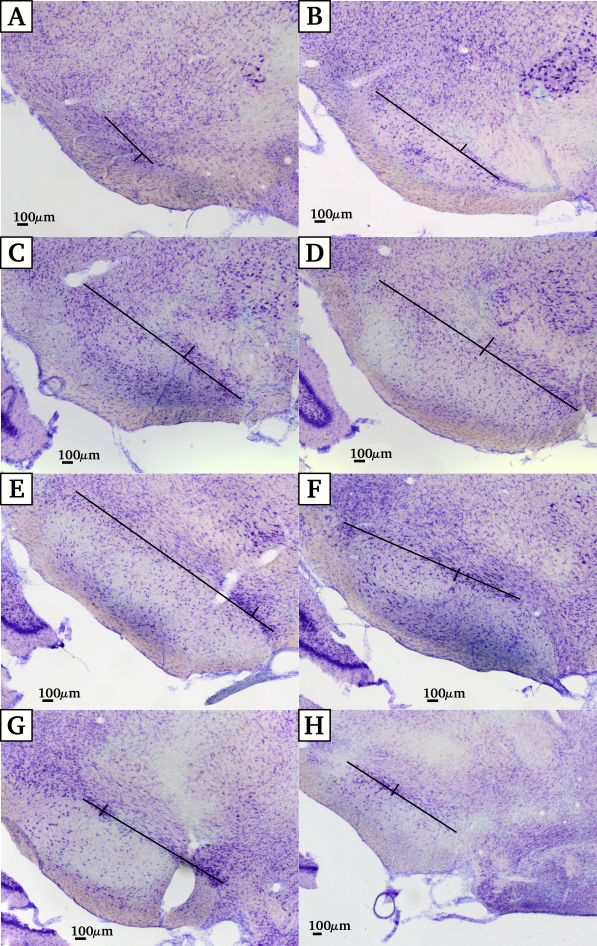
\includegraphics[width = 0.9\textwidth]{pictures/Bilder_monoamine_systeme/SNC.png}
    \caption[Substantia nigra pars compacta]{\textbf{Substantia nigra pars compacta.} Verlauf der pars compacta innerhalb des Mesencephalons von caudal (A: N16-1) nach rostral (H: N19-3).}
    \label{fig:SNC}
\end{figure}

\begin{table}[H]
\centering
\caption[Volumen der Substantia nigra]{\textbf{Volumen der Substantia nigra.} Es wurde die Länge und Breite der Substantia nigra pars compacta in den acht Nissl-Schnitten in Abbildung~\ref{fig:SNC} ausgemessen. Die Höhe wurde von einem Schnitt bis zum nächsten ausgemessenen Schnitt genommen. Die letzte Zeile zeigt die jeweilige Summe der Spalte.
Insgesamt hat die Substantia nigra pars compacta unserer Ratte ein Volumen von 0.5211~mm\textsuperscript{3}}
\label{tab:Volumen_SNC}
\resizebox{\textwidth}{!}{%
\begin{tabular}{cccccc}
\multicolumn{1}{l}{\textbf{Bild}} & \multicolumn{1}{l}{\textbf{Länge ($\upmu$m)}} & \multicolumn{1}{l}{\textbf{Breite ($\upmu$m)}} & \multicolumn{1}{l}{\textbf{Höhe ($\upmu$m)}} & \multicolumn{1}{l}{\textbf{Volumen ($\upmu$m\textsuperscript{3})}} & \multicolumn{1}{l}{\textbf{Volumen (mm\textsuperscript{3})}} \\ \hline
A                                 & 620.41                                  & 104.68                                   & 300                                    & 19483355.64                                & 0.0195                                     \\
B                                 & 1385.95                                 & 97.18                                    & 300                                    & 40405986.3                                 & 0.0404                                     \\
C                                 & 1792.57                                 & 156.31                                   & 300                                    & 84058985.01                                & 0.0841                                     \\
D                                 & 2183.08                                 & 212.78                                   & 300                                    & 139354728.72                               & 0.1394                                     \\
E                                 & 2227.12                                 & 108.85                                   & 300                                    & 72726603.6                                 & 0.0727                                     \\
F                                 & 1766.44                                 & 124.86                                   & 300                                    & 66167309.52                                & 0.0662                                     \\
G                                 & 1506.72                                 & 120.33                                   & 300                                    & 54391085.28                                & 0.0544                                     \\
H                                 & 1197.16                                 & 123.93                                   & 300                                    & 44509211.64                                & 0.0445                                     \\\hline
                                  &                                 &                                   & 2400                                   & 521097265.71                               & \textbf{0.5211}                           
\end{tabular}%
}
\end{table}


\subsubsection{Größenvergleich der Neurone in der Substantia nigra und im Locus coeruleus}

\begin{figure}[H]
    \centering
    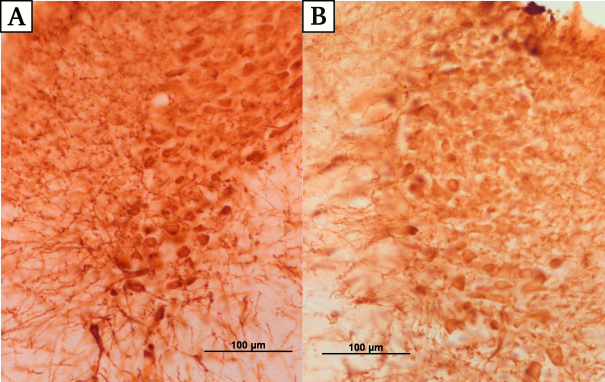
\includegraphics{pictures/Bilder_monoamine_systeme/Zellen_LC.png}
    \caption[Zellen des Locus coeruleus]{\textbf{Zellen des Locus coeruleus.} Nahaufnahme angefärbten Zellen des Locus coeruleus in den immunhistochemischen (TH-Nachweis) Schnitten. \textbf{A}: (Ia05-2), \textbf{B}: (Ib05-2). Insgesamt wurden 50 Somata in den beiden Schnitten ausgemessen. Im Mittel haben die Somata des Locus coeruleus einen Durchmesser 12.10~$\upmu$m~\rpm~0.1}
    \label{fig:Zellen_LC}
\end{figure}

\newpage
In den immunhistochemischen Schnitten konnte beim Locus coeruleus \index{Locus coeruleus} in zwei Schnittebenen (Abb.~\ref{fig:Zellen_LC}) über 150~$\upmu$m hinweg bei 50 Somata der Durchmesser ausgemessen werden. Im Durchschnitt ist der Durchmesser der Somata im Locus coeruleus 12.10~$\upmu$m~\rpm0.1 weit. Dabei war die kleinste Zelle 7.3~$\upmu$m breit und die größte Zelle 20.18~$\upmu$m breit.
\\
\\
Für die Substantia nigra pars compacta \index{Substantia nigra} wurden in drei Schnittebenen (Abb.~\ref{fig:Zellen_SNC}) über 600~$\upmu$m hinweg, ebenfalls bei 50 Somata, der Durchmesser bestimmt. Im Durchschnitt ist der Durchmesser der Somata in der Substantia nigra 14.78~$\upmu$m~\rpm0.09 weit. Die kleinste gemessene Zelle war im Durchmesser 10.61~$\upmu$m breit und die größte gemessene 20.25~$\upmu$m breit.

Die Zellen in den beiden Kerngebieten unterscheiden sich in ihrer Größe signifikant (t-Test, T(98) = 5.45, p $<$ 0.001) voneinander.

\begin{figure}[H]
    \centering
    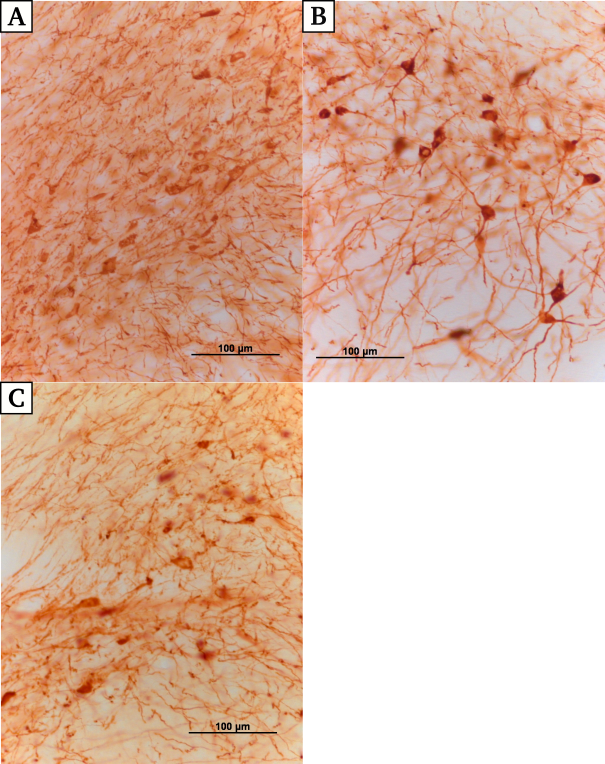
\includegraphics{pictures/Bilder_monoamine_systeme/Zellen_SNC.png}
    \caption[Zellen des Substantia nigra pars compacta]{\textbf{Zellen des Substantia nigra pars compacta.} Nahaufnahme angefärbter Zellen der Substantia nigra pars compacta in den immunhistochemischen (TH-Nachweis) Schnitten. \textbf{A}: (Ib08-1), \textbf{B}: (Ib08-2), \textbf{C}: (Ib08-3). Insgesamt wurden 50 Somata in den Schnitten ausgemessen. Im Mittel haben die Somata der Substantia nigra pars compacta einen Durchmesser von 14.78~$\upmu$m~\rpm~0.09}
    \label{fig:Zellen_SNC}
\end{figure}

\begin{comment}
50 Neurone in beiden Kerngebieten
LC : mean = 12.10 \rpm 0.1
SNC: mean = 14.78 \rpm 0.09
t.test: T(98) = 5.45174646; p < 0.001
\end{comment}

